\begin{center}

\begin{tikzpicture}[font=\small,overlay,
mycirclex/.style={draw, circle, minimum size=1.0em, inner sep = 0.2mm}, 
mydiamond/.style={draw, diamond, minimum size=0.78em, inner sep = 0mm}, 
myrectang/.style={draw, rectangle, minimum size=0.60em, inner sep = 0mm}, 
>=stealth]

\def\cola{blue} 
\def\colb{orange}
\def\colc{mygreen}
\def\cold{purple} 
\def\cole{gray} 
\def\colf{cyan}
\def\colg{brown}


\def\len{1.15cm}


% G1
\begin{scope}[local bounding box=bbox, xshift=-3.6cm]
\path<1-> node[mycirclex] (vs) at ( -1 * \len, 0) {$s$};
\path<1-> node[mycirclex] (v0) at (0.0 * \len, 0) {$a$};
\path<1-> node[mycirclex] (v1) at (1.0 * \len, 0) {$b$};
\path<1-> node[mycirclex] (v2) at (2.0 * \len, 0) {$c$};
\path<1-> node[mycirclex] (v3) at (3.0 * \len, 0) {$d$};
\path<1-> node[mycirclex] (v4) at (4.0 * \len, 0) {$e$};
\path<1-> node[mycirclex] (v5) at (5.0 * \len, 0) {$f$};
\path<1-> node[mycirclex] (v6) at (6.0 * \len, 0) {$g$};
\path<1-> node[mycirclex] (v7) at (7.0 * \len, 0) {$t$};

\path<1-> [draw, \colx, ->, line width=0.04cm] (vs) -- (v0);
\path<1-> [draw, \colx, ->, line width=0.04cm] (v0) -- (v1);
\path<1-> [draw, \colx, ->, line width=0.04cm] (v1) -- (v2);
\path<1-> [draw, \colx, ->, line width=0.04cm] (v2) -- (v3);
\path<1-> [draw, \colx, ->, line width=0.04cm] (v3) -- (v4);
\path<1-> [draw, \colx, ->, line width=0.04cm] (v4) -- (v5);
\path<1-> [draw, \colx, ->, line width=0.04cm] (v5) -- (v6);
\path<1-> [draw, \colx, ->, line width=0.04cm] (v6) -- (v7);

\path<1-> [draw, \colx, ->, line width=0.04cm, bend left = 40] (vs) to (v1);
\path<1-> [draw, \colx, ->, line width=0.04cm, bend left = 40] (v0) to (v2);
\path<1-> [draw, \colx, ->, line width=0.04cm, bend left = 40] (v2) to (v4);
\path<1-> [draw, \colx, ->, line width=0.04cm, bend left = 40] (v4) to (v6);
\path<1-> [draw, \colx, ->, line width=0.04cm, bend left = 40] (v5) to (v7);
\path<1-> [draw, \colx, ->, line width=0.04cm, bend left = 40] (v2) to (v7);

\path<1-> node[\colx] at (-.5 * \len, 0.15cm) {$e_1$};
\path<1-> node[\colx] at (0.5 * \len, 0.15cm) {$e_2$};
\path<1-> node[\colx] at (1.5 * \len, 0.15cm) {$e_3$};
\path<1-> node[\colx] at (2.5 * \len, 0.15cm) {$e_4$};
\path<1-> node[\colx] at (3.5 * \len, 0.15cm) {$e_5$};
\path<1-> node[\colx] at (4.5 * \len, 0.15cm) {$e_6$};
\path<1-> node[\colx] at (5.5 * \len, 0.15cm) {$e_7$};
\path<1-> node[\colx] at (6.5 * \len, 0.15cm) {$e_8$};

\path<1-> node[\colx] at (0.0 * \len, 0.65cm) {$e_9$};
\path<1-> node[\colx] at (1.0 * \len, 0.65cm) {$e_{10}$};
\path<1-> node[\colx] at (3.0 * \len, 0.65cm) {$e_{11}$};
\path<1-> node[\colx] at (5.0 * \len, 0.65cm) {$e_{12}$};
\path<1-> node[\colx] at (6.0 * \len, 0.65cm) {$e_{13}$};
\path<1-> node[\colx] at (4.5 * \len, 1.30cm) {$e_{14}$};

\end{scope}
%\path<1-> [draw, rounded corners] ($(bbox.south west) - (0.00cm, 0.25cm)$) rectangle ($(bbox.north east) + (0.1cm, 0)$);
%\node at ($(bbox.south) - (0.00cm, 0.2cm)$) [label=below:{$G_2 - G_1 = \{c\}$}]{};

\path<1-> [draw, line width=0.1cm, ->] (-0.15cm, -0.4cm) -- (-0.15cm, -1.0cm);

% G2
\begin{scope}[local bounding box=bbox, xshift=-3.6cm, yshift=-2.0cm]
\path<1-> node[mycirclex] (vs) at ( -1 * \len, 0) {$s$};
\path<1-> node[mycirclex] (v0) at (0.0 * \len, 0) {$a$};
\path<1-> node[mycirclex] (v1) at (1.0 * \len, 0) {$b$};
\path<1-> node[mycirclex] (v2) at (2.0 * \len, 0) {$c$};
\path<1-> node[mycirclex] (v3) at (3.0 * \len, 0) {$d$};
\path<1-> node[mycirclex] (v4) at (4.0 * \len, 0) {$e$};
\path<1-> node[mycirclex] (v5) at (5.0 * \len, 0) {$f$};
\path<1-> node[mycirclex] (v6) at (6.0 * \len, 0) {$g$};
\path<1-> node[mycirclex] (v7) at (7.0 * \len, 0) {$t$};

\path<1-> [draw, \colx, ->, line width=0.04cm] (vs) -- (v0);
\path<1-> [draw, \colx, ->, line width=0.04cm] (v0) -- (v1);
\path<1-> [draw, \colx, ->, line width=0.04cm] (v1) -- (v2);
\path<1-> [draw, \colx, ->, line width=0.04cm] (v2) -- (v3);
\path<1-> [draw, \colx, ->, line width=0.04cm] (v3) -- (v4);
\path<1-> [draw, \colx, ->, line width=0.04cm] (v4) -- (v5);
\path<1-> [draw, \colx, ->, line width=0.04cm] (v5) -- (v6);
\path<1-> [draw, \colx, ->, line width=0.04cm] (v6) -- (v7);

\path<1-> [draw, \colx, ->, line width=0.04cm, bend left = 40] (vs) to (v2);
\path<1-> [draw, \colx, ->, line width=0.04cm, bend left = 40] (v2) to (v4);
\path<1-> [draw, \colx, ->, line width=0.04cm, bend left = 40] (v4) to (v7);
\path<1-> [draw, \colx, ->, line width=0.04cm, bend left = 40] (v2) to (v7);

\path<1-> node[\colx] at (-.5 * \len, 0.15cm) {$e_1$};
\path<1-> node[\colx] at (0.5 * \len, 0.15cm) {$e_2$};
\path<1-> node[\colx] at (1.5 * \len, 0.15cm) {$e_3$};
\path<1-> node[\colx] at (2.5 * \len, 0.15cm) {$e_4$};
\path<1-> node[\colx] at (3.5 * \len, 0.15cm) {$e_5$};
\path<1-> node[\colx] at (4.5 * \len, 0.15cm) {$e_6$};
\path<1-> node[\colx] at (5.5 * \len, 0.15cm) {$e_7$};
\path<1-> node[\colx] at (6.5 * \len, 0.15cm) {$e_8$};

\path<1-> node[\colx] at (0.5 * \len, 0.88cm) {$e_{15}$};
\path<1-> node[\colx] at (3.0 * \len, 0.65cm) {$e_{11}$};
\path<1-> node[\colx] at (5.5 * \len, 0.88cm) {$e_{16}$};
\path<1-> node[\colx] at (4.5 * \len, 1.30cm) {$e_{14}$};

\end{scope}
%\path<1-> [draw, rounded corners] ($(bbox.south west) - (0.00cm, 0.25cm)$) rectangle ($(bbox.north east) + (0.1cm, 0)$);
%\node at ($(bbox.south) - (0.00cm, 0.2cm)$) [label=below:{$G_2 - G_1 = \{c\}$}]{};


\end{tikzpicture}
\end{center}
